% !TEX root = paper.tex

\section {Results}
\label{sec:results}
\subsection{Transverse-momentum and multiplicity dependence of anisotropic flow}

\begin{figure}[!b]
	\centering
	\hspace{-3em}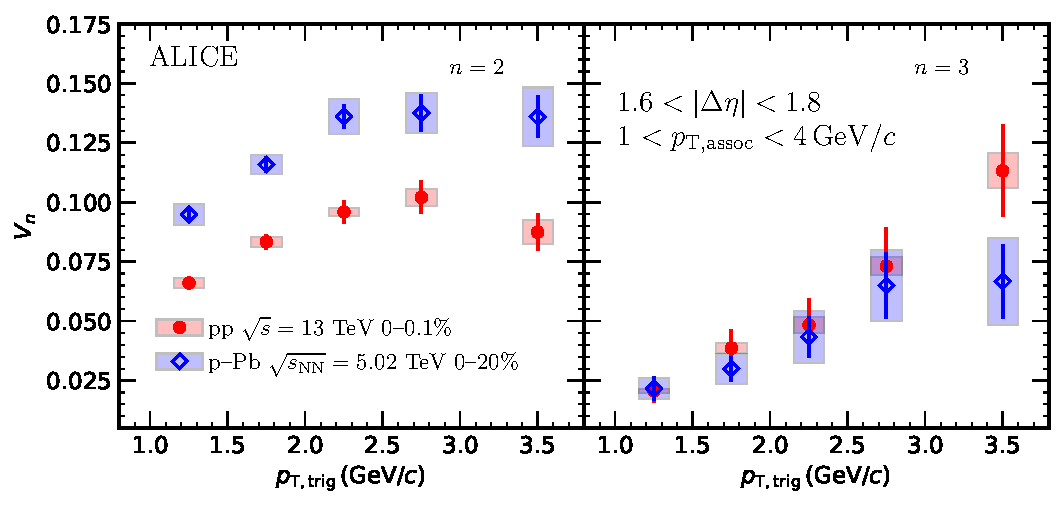
\includegraphics[width=0.9\textwidth]{figures/FIG4_vn_pppPb.pdf} %<--- keep the scale at 0.9 to match with other figures
	\caption{The magnitude of $v_2$ (left) and $v_3$ (right) as a function of $p_\mathrm{T}$ for the high-multiplicity interval of the 0--0.1\% in pp collisions at $\sqrt{s}=13$~TeV and 0--20\% in p--Pb collisions at $\sqrt{s_\mathrm{NN}} = 5.02$~TeV. The boxes around the data points describes the systematic uncertainty estimation and the lines corresponds to the statistical uncertainty.}
	\label{fig:vn}
\end{figure}
%python3 Fig2_vn_ppPb.py
Figure~\ref{fig:vn} illustrates the extracted values of $v_2$ and $v_3$ as functions of $p_{\mathrm{T,trig}}$ using Eq.~\ref{eq:tmpfit}. The results were obtained from the high-multiplicity interval of 0--0.1\% in pp collisions at $\sqrt{s}=13$TeV and 0--20\% in p--Pb collisions at $\sqrt{s_\mathrm{NN}}=$5.02~TeV. Both sets of results demonstrate an increasing trend in the magnitudes of $v_n$ as $p_{\mathrm{T,trig}}$ rises, peaking between $2.5<p_{\mathrm{T,trig}}<3.0$ GeV/c for $v_2$ within the limit of errors, akin to the observations in Pb--Pb collisions\cite{Abelev:2012di, ALICE:2018yph}.
The magnitudes of $v_2$ in p--Pb collisions are higher than those in pp collisions, which might be related to the larger system size in p--Pb together with a likely longer lifetime of the hypothetically created medium.
However, the magnitudes of $v_3$ are similar in both systems, indicating that $v_3$ is less sensitive to the size of the systems.
These results are comparable to those obtained by ATLAS in different multiplicity classes, where the same method was used to extract the flow coefficients~\cite{ATLAS:2016yzd}. Even though the $\Delta\eta$ and $p_{\mathrm{T,assoc}}$ ranges are wider in the ATLAS results, $2.0<|\Delta\eta|<5.0$ and $0.5<p_{\mathrm{T,assoc}}<5\,\mathrm{GeV}/c$, respectively, the results are consistent within uncertainties.

\begin{figure}[!t]
	\centering
%python3 Fig6_vn_allSystems_comp_dataonly.py
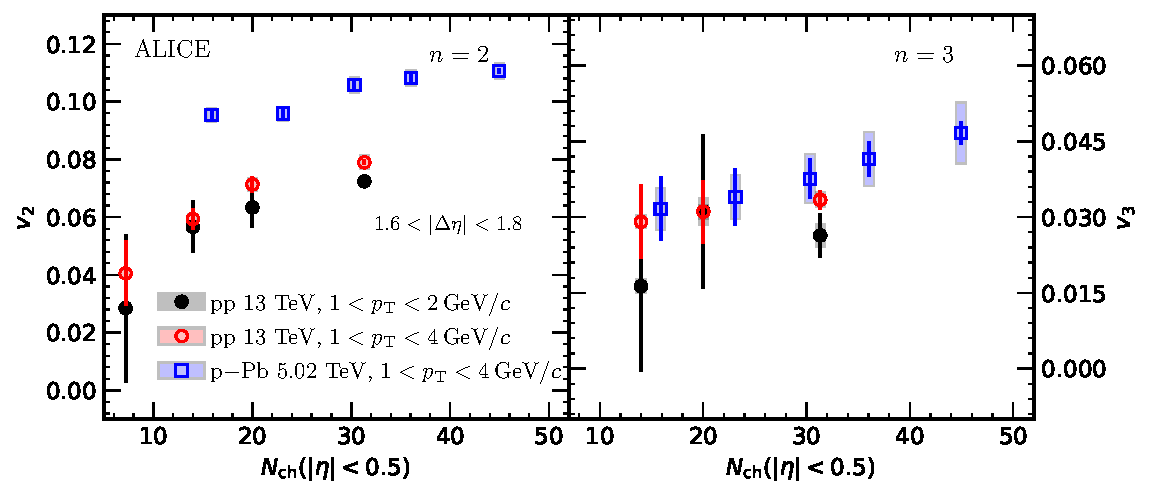
\includegraphics[width=1.0\textwidth]{figures/FIG5_v2Mult_allSystems_Data.pdf} 
	\caption{The magnitudes of $v_2$ (left
    panel) and $v_3$ (right panel) 
 for two different collision systems, pp and p--Pb as a function of charged-particle multiplicity at midrapidity. For pp collisions, two different $p_\mathrm{T}$-intervals are shown, $1.0<p_\mathrm{T}<2.0$ GeV/c and $1.0<p_\mathrm{T}<4.0$ GeV/$c$. The boxes around the data points describes the systematic uncertainty estimation and the lines corresponds to the statistical uncertainty.} 
	\label{fig:v2mult}
\end{figure}

Figure~\ref{fig:v2mult} presents the magnitudes of $v_2$ and $v_3$, as functions of charged-particle multiplicity in the midrapidity ($N_{ch}$ ($|\eta|<0.5$)) for both pp collisions at $\sqrt{s}=13$ TeV and p--Pb collisions at $\sqrt{s_\mathrm{NN}}=5.02$ TeV. As in Fig.~\ref{fig:vn}, the $\Delta\eta$ gap is considered at $1.6<|\Delta\eta|<1.8$ and $v_2$ is measured in $1<p_{\mathrm{T}}<4\,\mathrm{GeV}/c$ for both collision systems. Additionally, the corresponding results for pp collisions at $\sqrt{s}=13$ TeV with $1<p_{\mathrm{T}}<2$ GeV/$c$ are presented. First, it is observed that the magnitude of $v_n$ increases with increasing multiplicity for both collision systems and $p_\mathrm{T}$-ranges. Second, $v_2$ in p--Pb is higher than in pp collisions in the measured multiplicity range. These two observations are compatible with previous results from Refs.~\cite{ATLAS:2015hzw,ATLAS:2016yzd, Khachatryan:2015lva}. There is no significant difference between two collision systems in $v_3$ dependence on multiplicity as shown on the right-hand side panel of Fig.~\ref{fig:v2mult}. The $v_3$ measurements exhibit a comparable, subtle dependence on multiplicity, with higher values observed in collisions with greater particle multiplicities.
For the two different $p_\mathrm{T}$ intervals presented for the pp collisions, the $v_2$ in $1.0<p_\mathrm{T}<4.0$ GeV/$c$ shows a hint of larger magnitude than the $v_2$ in $1.0<p_\mathrm{T}<$~2.0~GeV/$c$. The difference in magnitude is significant only in the highest multiplicity point. 
This agrees with what is observed in Fig.~\ref{fig:vn}, where the $v_2$ magnitude has its largest value in $2.5<p_\mathrm{T}<$~3.0~GeV/$c$. It is found that for the considered $p_\mathrm{T}$ selections, the observed multiplicity dependencies differ only marginally. 
It is worth noting that the results presented for pp and p--Pb collisions were obtained from two different beam energies. In \cite{ATLAS:2016yzd}, it was found that the magnitudes of $v_2$ and $v_3$ in pp collisions between 13 and 5.02 TeV show no significant variation with center-of-mass energy.

\subsection{Event-scale dependence of the flow coefficients}
\begin{figure}[h!]
	\centering
	\hspace{-3em}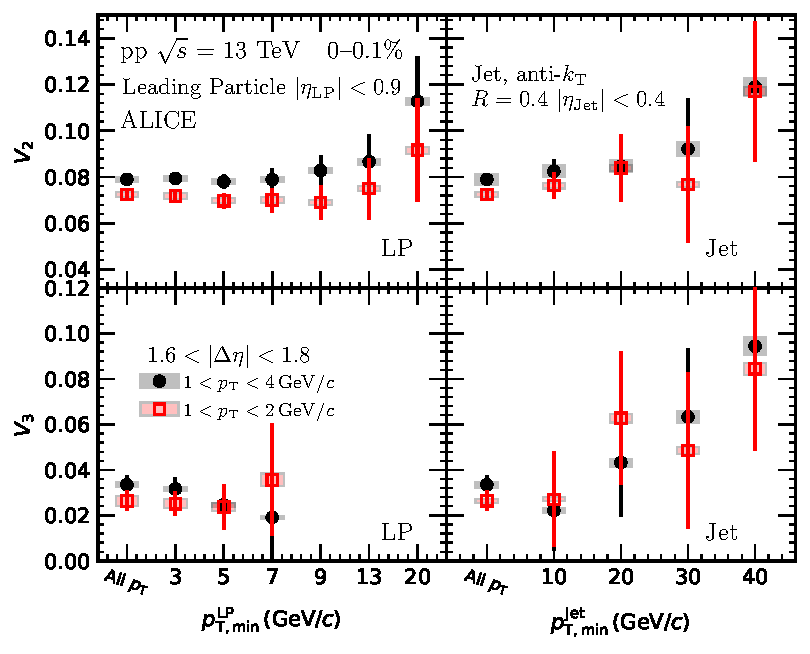
\includegraphics[width=0.8\textwidth]{figures/FIG6_vn_LP.pdf}
	\caption{The magnitudes of $v_2$ (top) and $v_3$ (bottom) as a function of the $\it{p}^{\rm{LP}}_{\rm{T,min}}$ (left) and $\it{p}^{\rm{jet}}_{\rm{T,min}}$ (right) for the high-multiplicity interval of the 0--0.1\% in pp collisions at $\sqrt{s}=13$. The measured $p_{\mathrm{T}}$ intervals are $1<p_{\mathrm{T}}<2\,\mathrm{GeV}/c$ (in red) and $1<p_{\mathrm{T}}<4\,\mathrm{GeV}/c$ (in black). The statistical and systematic uncertainties are shown as vertical bars and boxes, respectively.}
	\label{fig:LPjet23}
\end{figure}    

Figure~\ref{fig:LPjet23} presents the extracted magnitude of $v_2$ and $v_3$ as a function of the minimum $p_\mathrm{T}$ of the leading particle $\it{p}^{\rm{LP}}_{\rm{T,min}}$ and that of the jet ($\it{p}^{\rm{jet}}_{\rm{T,min}}$) as introduced in Section~\ref{sec:intro}. 
Both event-scale results are obtained from pp collisions at $\sqrt{s}= 13$ TeV for the 0--0.1\% multiplicity class and for two different $p_\mathrm{T}$-ranges.
To reduce the impact of the detector edge effects on the jet measurements, the jets are required to have a pseudorapidity $|\eta|<0.4$, following a similar approach as in Refs.~\cite{CDF:2001onq, ATLAS:2014riz, CMS:2015jdl}. The $v_2$ and $v_3$ values for both $p_\mathrm{T}$ ranges do not show any dependence on event-scale selection within the uncertainties. This finding is consistent with the results of the ridge yields~\cite{ALICE:2021nir} and $v_{2}$ measurements with a tagged $Z$ boson from the ATLAS collaboration~\cite{Aaboud:2019mcw}. These results suggest that the presence of a hard-scattering process does not significantly change the long-range correlation involving soft particles.
However, the presented measurements are only limited to the low $\it{p}^{\rm{jet}}_{\rm{T}}$. Future measurements with multi-jet events at midrapidity with higher $Q^2$ reach can shed more light on the expected impact parameter dependence~\cite{Sjostrand:1986ep,Frankfurt:2003td,Frankfurt:2010ea}.

\subsection{Comparisons with models}
\label{sec:theory}

\begin{figure}[h!]
	\centering
	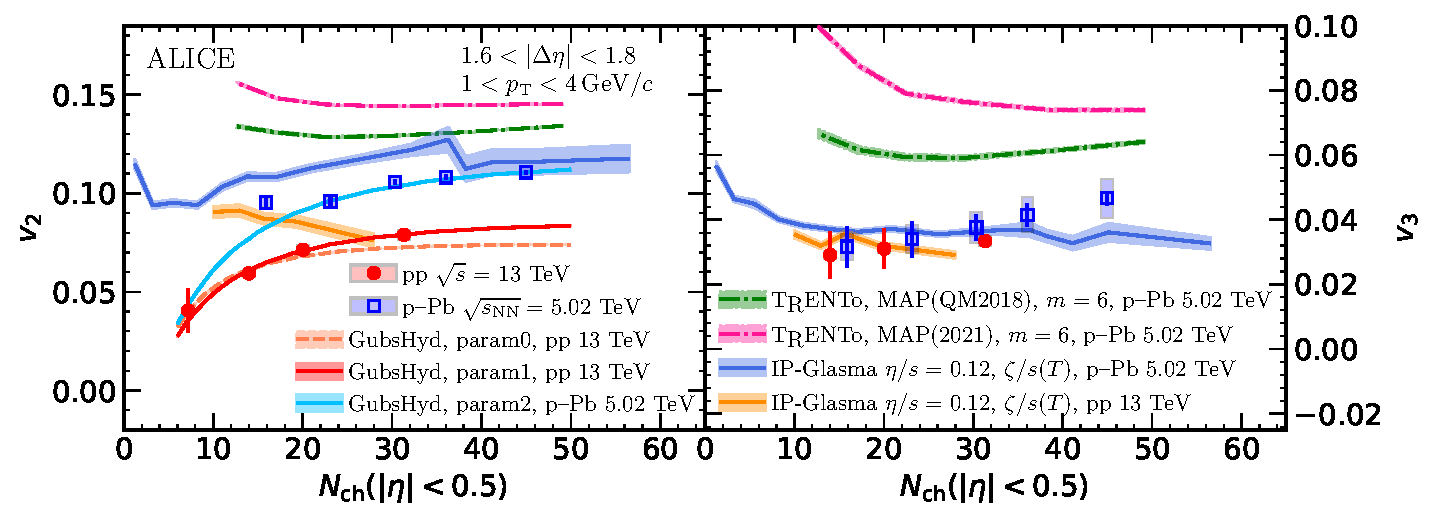
\includegraphics[width=1.0\textwidth]{figures/FIG7_v2Mult_allSystems_Hydro.pdf} 
	\caption{The measured and calculated evolution of $v_2$ (left) and $v_3$ (right) in pp and p--Pb collisions as a function of charged-particle multiplicity at midrapidity. The calculations are provided by hydrodynamical models~\cite{Parkkila:2021yha,Bernhard:2016tnd,Schenke:2020mbo,Taghavi:2019mqz}. Measured data are represented by markers and the calculations by bands.
    The blue and red markers represent the p--Pb and pp collision data points, respectively. The hydrodynamic calculations are presented with colored lines and bands marking their statistical uncertainty.} 
	\label{fig:vnmult_model}
\end{figure}

In this section, the results are compared to various model calculations.
The results from the data in p--Pb collisions are compared with hydrodynamic calculations using the parametrization from an improved global
Bayesian analysis of new sophisticated collective flow observables
 from two different beam energies in Pb--Pb collisions~\cite{Parkkila:2021yha}. This hydrodynamic model, {T\raisebox{-.5ex}{R}ENTo}+iEBE-VISHNU, consists of the {T\raisebox{-.5ex}{R}ENTo} model~\cite{Moreland:2014oya} for the initial condition, which is connected with a free streaming to a 2+1 dimensional causal hydrodynamic model VISH2+1~\cite{Shen:2014vra}. The evolution is continued after hadronization with a hadronic cascade (UrQMD) model~\cite{Bass:1998ca,Bleicher:1999xi}. The initial conditions, the shear viscocity $\eta/s(T)$, the bulk viscosity $\zeta/s(T)$, and other free parameters of the hybrid model are extracted in a global Bayesian analysis.
A model calculation is performed using the best-fit parameterization for transport coefficients selected based on maximum a posteriori (MAP) for Pb--Pb collisions at $\sqrt{s_{\text{NN}}}=5.02$~TeV. Two different MAP values are used for the calculations. One is based on Ref.~\cite{Parkkila:2021yha} and is labeled as MAP(2021) in Fig.~\ref{fig:vnmult_model}. The other value, labeled as MAP(QM2018) in Fig.~\ref{fig:vnmult_model}, is from Ref.~\cite{Bernhard:2016tnd}. The parameterization for the initial conditions, which include a sub-nucleon structure with six constituent partons per nucleon ($m=6$), is taken from a model calibration with additional p--Pb data~\cite{Moreland:2018gsh}. All kinematic selections, such as the transverse momentum and pseudorapidity intervals, are matched to the data reported in this article. The flow coefficients in the hydrodynamic calculation are extracted with the two-particle cumulant method, as those models do not contain any non-flow.

Figure~\ref{fig:vnmult_model} shows that {T\raisebox{-.5ex}{R}ENTo}+iEBE-VISHNU overestimates both $v_2$ and $v_3$. The data shows a dependence on multiplicity, with increasing values towards larger multiplicities in the predicted ranges. However, {T\raisebox{-.5ex}{R}ENTo}+iEBE-VISHNU predicts low values at higher multiplicities and higher values at low multiplicities, similar to what is found in large collision systems~\cite{Acharya:2020taj}. The large discrepancies in the prediction might be alleviated by inclusion of the newly measured p--Pb constraints in a future Bayesian parameter estimation as well as by improvements of the initial condition model for the small-system collisions.

The results are also compared with IP-Glasma+MUSIC+UrQMD hydrodynamic calculations~\cite{Schenke:2020mbo}. This model uses IP-Glasma initial conditions~\cite{Schenke:2012wb} including sub-nucleonic fluctuations with three hot-spots per nucleon. The hydrodynamic evolution is performed by MUSIC~\cite{Schenke:2010rr} and coupled with UrQMD~\cite{Bass:1998ca,Bleicher:1999xi} for the hadronic cascade. 
The model calculations are performed assuming constant $\eta/s=0.12$ and a temperature dependent $\zeta/s(T)$~\cite{Rose:2020lfc}. 
This model describes well the multiplicity dependence of $v_2$ in p--Pb collisions and the magnitude at the highest multiplicity within the statistical uncertainties of the model but overestimates the data for the lower multiplicity classes. As for pp collisions, the calculations clearly miss both the observed magnitude except for $N_\mathrm{ch}>25$ as well as the trend of the multiplicity dependence. The model shows that $v_2$ decreases with increasing multiplicity, while the experimental result shows the opposite.
For $v_3$, the model accurately describes the magnitudes and multiplicity dependence across the measured multiplicity ranges. The magnitudes of $v_3$ are slightly smaller in pp collisions than in p--Pb collisions according to the calculations, which agrees with the data within the uncertainties. The findings involving this model are consistent with the comparison done in Ref.~\cite{Acharya:2019vdf}.

Finally, the results are compared with the GubsHyd model, a semi-analytical model based on the analytical Gubser solution to hydrodynamic equations~\cite{Gubser:2010ze,Gubser:2010ui}, known as Gubser flow. In Gubser flow, the initial state of a conformal matter is linearly perturbed by an initial elliptic shape. The model is employed to shed light on the possible sources of the observed discrepancy between more realistic models mentioned above and the measurements in pp collisions~\cite{Taghavi:2019mqz}. Instead of modeling the initial entropy density in this model, as it is typically done in T$_{\text{R}}$ENTo or IP-Glasma, the initial state fluctuation is modeled directly. It assumes that proton ellipticity $\epsilon_{2}$ and RMS radius $r_{\text{rms}}$ fluctuate independently. These fluctuations are described by probability distributions, which have widths $\sigma_{\epsilon}$
 and $\sigma_{r}$, respectively. The multiplicity dependence of two-particle correlation functions' $v_2\{2\}$ depends on $\sigma_{r}$ and  $\chi\sigma_{\epsilon}$, which can be obtained by comparing the model with data. Since no non-flow effect is considered in the calculation, $v_2\{2\}$ is comparable with the flow measurements in the present study. The coefficient $\chi$ encapsulates the correction to all the idealization of GubsHyd, including the absence of dissipation effects. The calculations for two sets of parameters are compared
to data in Fig.~\ref{fig:vnmult_model}. The “param0” parameterization is based on the prediction proposed in Ref.~\cite{Taghavi:2019mqz} that $\chi \sigma_{\epsilon} =$ 0.097 and $\sigma_{r} =$ 0.4 fm. The other parameterizations “param1” and “param2” employ different $\chi \sigma_{\epsilon}$  and $\sigma_{r}$ values. The model captures the multiplicity dependence of $v_2$ well.

The measured value of $v_{2}$ decreases with decreasing multiplicity in both pp and p--Pb collisions. This trend is also predicted by GubsHyd model calculations (Refs.~\cite{Taghavi:2019mqz} and~\cite{Weller:2017tsr}). Interestingly, the opposite trend is observed for the IP-GLASMA+MUSIC+UrQMD hydrodynamic calculations of $v_2$, where the value decreases with increasing charged-particle multiplicity~\cite{Schenke:2020mbo}.
Approaching a lower bound for the size of a hydrodynamized
system as predicted in Ref.~\cite{Taghavi:2019mqz}, 
the decreasing trend of $v_2$, obtained by lowering the charged-particle multiplicity, changes and turns out to raise again after the observed minimum. However, this change in multiplicity dependence of $v_2$ at low multiplicities is still challenging to test with the current experimental uncertainties. For $v_3$, the IP-Glasma+MUSIC+UrQMD hydrodynamic calculations~\cite{Schenke:2020mbo} are the only ones that accurately describe its magnitude and multiplicity dependence across the measured ranges. The calculations predict that the magnitudes of $v_3$ are slightly smaller in pp collisions than in p--Pb collisions, within the measured multiplicity ranges. The discrepancies between the predictions and the data can be further studied by including these measurements in a future Bayesian parameter estimation, as well as by improving the initial-condition model for the small-system collisions.